\documentclass{scrartcl}
\title{\rmfamily Software Engineering -- Blatt 10}
\author{Rasmus Diederichsen \and Felix Breuninger\and 
   \texttt{\{rdiederichse, fbreunin\}@uos.de}
}
\date{\today}
\usepackage[ngerman]{babel}
\usepackage[space]{grffile} % for spaces in includegraphics fnames
\usepackage{marvosym, microtype, textcomp, xifthen, multirow, booktabs, dingbat,
   titlesec, enumitem, fullpage, tikz, IEEEtrantools, array, amsmath, listings,
   colortbl,
amssymb, graphicx, subcaption, lmodern,pgfplots}
\usepackage[pdftitle={Software Engineering -- Blatt 10}, 
   pdfauthor={Rasmus Diederichsen, Felix Breuninger}, 
   hyperfootnotes=true,
   colorlinks,
   bookmarksnumbered = true,
   linkcolor = lightgray,
   plainpages = false,
citecolor = lightgray]{hyperref}
\usepackage[utf8]{inputenc}
\usepackage[T1]{fontenc}
\usepackage[all]{hypcap}
\titleformat{\section}[hang]{\bf}{Aufgabe 10.\arabic{section}:}{1em}{}[]
\titleformat{\subsection}[hang]{\bf}{\hspace{1em}\alph{subsection})}{1em}{}[]

\lstset{
   frame=single,
   basicstyle=\ttfamily\small,
   frameround=tttt,
   backgroundcolor=\color{lightgray!10},
   keywordstyle=\color{teal}\textbf,
   stringstyle=\itshape,
   showstringspaces=false,
   language=[gnu] make,
   morecomment=[n]{$(}{)},
   commentstyle=\color{blue},
   title=\lstname
}
\usetikzlibrary{shapes,positioning,calc,decorations.text,graphs,arrows.meta}
\begin{document}

\fontfamily{ptm}\selectfont
\maketitle

\section{Evolutionäre / inkrementelle Modelle}

\subsection{Inkrementelle Modelle}

Der inkrementelle Entwicklungsprozess ist durch folgende Aspekte gekennzeichnet:
\begin{itemize}
   \item Software im Allgemeinen zunächst als Kernprodukt abgeliefert
   \item Nach und nach werden Features hinzugefügt
   \item Jedes Feature durchläuft einen kompletten Entwichklungszyklus (z.B. wie
      im Wasserfallmodell)
   \item Frühere Releases sind abgespeckte Versionen der späteren.
   \item Inkremente werden anhand der Benutzung des vorherigen Releases durch
      den Kunden durchgeplant unt entwickelt.
\end{itemize}

\newcolumntype{V}{>{\columncolor{green!10}\flushleft\arraybackslash}p{.4\textwidth}}
\newcolumntype{N}{>{\columncolor{red!10}\flushleft\arraybackslash}p{.4\textwidth}}
\begin{center}
   \begin{tabular}{VN}
      \toprule
      \textbf{Vorteile} & \textbf{Nachteile} \\ 
      \midrule
       Schneller Weg zur fertigen Kernfunktionalität & Unklar, wann es ``fertig'' ist \\
       Es werden keine Releases weggeworfen, Qualitätsarbeit in jeder Iteraion  & Inkremente v. A. nach User-Feedback $\rightarrow$ schwer planbar \\
       Entwicklung kann bei Einhaltung on Restriktionen dennoch stets fertiges
       Produkt liefern (Ressourcenknappheit, Deadlines, Warten auf Technologien,
       etc.) & \\
       Beliebige Erweiterbarkeit (potenziell langlebig) & \\
       Kurze Iterationen machen Fehler weniger teuer & \\
       Nachträgliche Ergänzungen einfach einzubauen & \\
   \end{tabular}
\end{center}

\begin{figure}
   {\centering      
   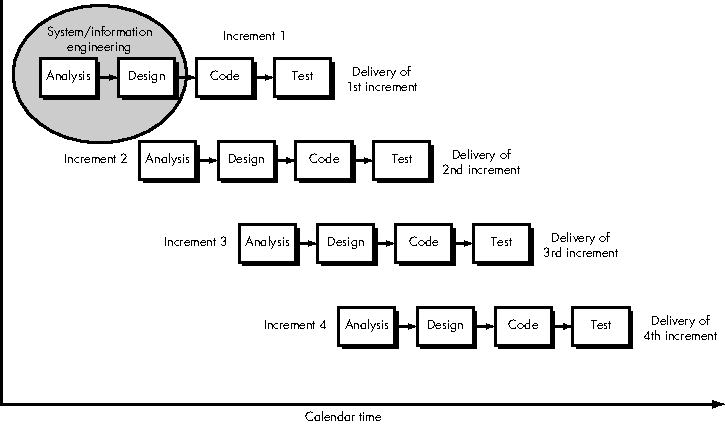
\includegraphics[width=\textwidth]{incremental_pressman.pdf}
   \caption{Iteratives Vorgehensmodell}
   \label{iter}}
\end{figure}

\subsection{Evolutionäre Modelle}

Das evolutionäre Vorgehen ist charakterisiert durch
\begin{itemize}
   \item Anforderungen, Pläne, Designs, Aufwandsschätzungen etc. entwickeln sich
      über die Zeit
   \item Entwicklung verläuft iterativ, indem die einzelnen Phasen nach
      Anpassung der Spezifikationen wiederholt werden
   \item In jeder Iteration werden die Bestandteile der Phasen (s.o.) verfeinert 
   \item im Spiralmodell schreitet die Entwicklung spiralförmig fort, indem
      aufbauend auf dem Produkt der vorherigen Iteration immer alle Phasen neu
      durchlaufen werden.
   \item Anders als beim rein inkrementellen Vorgehen durchlaufen nicht einzelne
      Features den Entwicklungsprozess und werden ``angetackert'', sondern die
      Gesamtsofware wird überarbeitet.
\end{itemize}

\begin{center}
   \begin{tabular}{VN}
      \toprule
      \textbf{Vorteile} & \textbf{Nachteile} \\ 
      \midrule
      Hohe Anpassbarkeit an Kundenvorstellungen & Schwer planbar, da Anforderungen nicht zu Anfang bekannt\\
      Schneller Prototyp & Versionen werden verworfen \\
      Anforderungen müssen nicht alle zu Beginn bekannt sein & Häufige
      Änderungen sind schwer zu überblicken und können zu schlechterem Code
      führen \\
      Sämtliche Projektdokumente werden verbessert, alles ist konsistent & \\
      Prozess hat kein Ende, kann gesamte Lebensdauer abdecken & Kein klares
      Ende \\
      Zu keinem Zeitpunkt im Lebenszyklus werden Aspekte vernachlässigt. & \\
   \end{tabular}
\end{center}

\begin{figure}
   {\centering      
      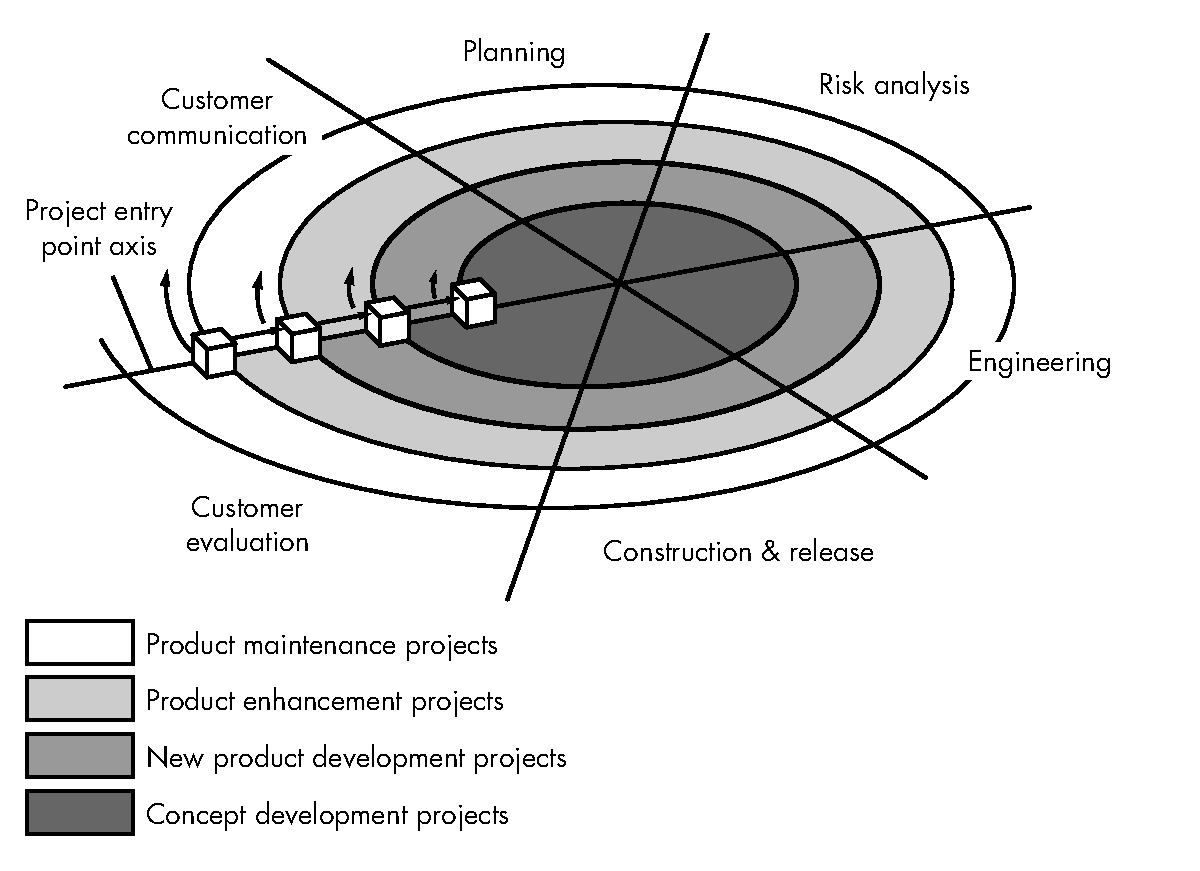
\includegraphics[width=\textwidth]{evol_pressman.pdf}
   \caption{Spiralmodell; Evolutionäres Vorgehen mit definierten Task Sets}
   \label{evo}}
\end{figure}

\vspace{\baselineskip}
\noindent\textbf{Quellen}:
\begin{enumerate}
   \item \emph{Pressman, R.: Software engineering: a practitioner’s approach, 5th ed.}
   \item \emph{Larman, C.: Agile and Iterative Development: A Manage's Guide}
\end{enumerate}

\section{Vorgehensmodelle}
\begin{enumerate}
   \item Da die Anforderungen bekannt sind und ein strikter Zeitplan möglich
      ist, bietes sich ein lineares Vorgehen wie Wasserfall oder V-Modell an.
      Es ist nicht erforderlich, möglichst schnell etwas präsentieren zu können,
      also muss man nicht agil vorgehen.
   \item Rapides Prototyping erlaubt, das Problem notdürftig zu hotfixen, der
      Fix kann dann verbessert und stabilisiert werden. Möglich wäre auch ein
      Code-and-Fix-Ansatz, da hier höchste Dringlichkeit gegeben ist.
   \item Evolutionär vorzugehen, würde es erlauben, die zwangsläufig
      auftretenden Änderungen miteinzubeziehen.
   \item Das V-Modell expliziert die Notwendigkeit und Zuständigkeit
      verschiedener Tests. Dank der vorliegenden älteren Version kann das
      Projekt gut von vorn bis hinten durchgeplant werden, bevor man anfängt.
   \item Code-and-Fix wäre hier ausreichend, da Dr. Blair kein
      Softwareingenieur ist und nur flott etwas demonstrieren muss. Die Software
      wird weder wirklich benötigt, noch wird sie länger in Betrieb sein.
\end{enumerate}

\section{Scrum}

\subsection{}

Zu Beginn des Projektes definiert der Kunde eine Menge von Funktionalitäten und
einen Zeitrahmen; die Funktionalitäten werden priorisiert und in das vom
\emph{Product Owner} gepflegte \emph{Product Backlog} eingefügt. Dies kann in
Form von User Stories mit assoziierten Story Points (Wichtigkeit, Aufwand) o.Ä.
geschehen. In einem \emph{Release Plan} wird dann die Dauer der Sprints und die
grobe Verteilung der Features festgehalten.

Anhand des Zeitrahmens kann die Zahl an Features, die im nächsten
\emph{Sprint} abgearbeitet werden sollen, sowie die Länge der Sprints (typisch
1-4 Wochen), festgelegt werden. Für jeden Sprint werden die wichtigsten Features
durch den Product Owner aus dem Product Backlog in das \emph{Sprint Backlog}
eingefügt und in dem für einen Sprint allokierten Zeitrahmen abgearbeitet. Das
Entwicklerteam hält täglich ein \emph{Daily Scrum} Meeting, in dem jedes Mitglied
folgende Fragen beantwortet:

\begin{enumerate}
   \item Was habe ich seit dem letzten Meeting erreicht?
   \item Welche Probleme traten dabei auf?
   \item Was werde ich bis zum nächsten Meeting schaffen?
\end{enumerate}

Anhand der Antworten können der \emph{Scrum Master}, der auch die korrekte
Einhaltung des Vorgehens überwacht, und das Management z.B. die Größe des Sprint
Backlogs oder andere Projektparameter variieren. Nach jedem Sprint wird die
erreichte Funktionalität dem Kunden (oder allgemeiner \emph{Product Owner})
vorgestellt. Während jedes Sprints kann ein \emph{Burndown Chart} die Zahl noch
umszusetzender Story Points der Zeit im Sprint gegenüberstellen, sodass man
sieht, ob man die gesteckten Ziele erreicht oder nicht, wenn man genau so weiter
macht. Die Zahl noch zu erreichender Story Points nimmt idealerweise linear ab.

Analog dazu gibt es auch ein \emph{Release Burndown Chart}, das den
Gesamtfortschritt überwacht, sodass der Release Plan gegebenenfalls angepasst
werden kann.   

Probleme werden in das \emph{Impediment Backlog} eingetragen.

Der \emph{Product Owner} kann jederzeit neue Funktionalität fordern, diese wird
aber zunächst ins Product Backlog eingefügt und daher erst im nächsten Sprint
bearbeitet.

Ein Feature gilt als fertig, wenn es die durch den Kunden gegebene
\emph{Definition of Done} erfüllt.

\subsection{}

\begin{center}
   \begin{tabular}{p{.5\textwidth}p{.5\textwidth}}
      Manifest-Element & Unterstützung durch Scrum \\
      Individuals and interactions over processes and tools & Tägliche Meetings,
      keine strenge Vorschift, wie innerhalb eines Sprints vorzugehen ist \\
      Working software over comprehensive documentation & Nach jedem Sprint kann
      eine Zwischenversion präsentiert werden, es gibt nur eine Handvoll
      Dokumente (s.o.) \\
      Customer collaboration over contract negotiation & Reviews finden am Ende
      jedes Sprints statt, der Kunde kann jederzeit neue Anforderungen
      formulieren, es muss nicht alles ab Start fest stehen \\
      Responding to change over following a plan & Zwar werden Pläne erstellt,
      sind jedoch änderbar. Änderungen können zu Anfang jedes Sprints Rechnugn
      getragen werden.
   \end{tabular}
\end{center}

\subsection{}
\begin{description}
  \item[Entwickle iterativ:] Sprints
  \item[Überwache Erfüllung der Anforderungen:] Sprint reviews
  \item[Verfolge Änderungen:] Product Backlog Refinement
  \item[Schließe jeden Schritt mit Qualitätsprüfung ab:] Sprint reviews / DoD
  \item[Lerne von Fehlern:] Sprint Retrospective Meeting 
  \item[Arbeite nach Plan:] Sprint / Product backlog
\end{description}

\subsection{}
\begin{description}
  \item[Product backlog:]  Liste von Anforderungen die Umzusetzen sind. Anforderungen werden hier priorisiert und pro Sprint wird eine ausgewählte Anforderung komplett umgesetzt.
  \item[Burndown Chart:] Visualisierung von Fortschritt in Bezug auf Gesamtprojekt / Sprint
  \item[Definition of Done:] Kriterien und Anforderungen, wann eine Arbeit als fertig bezeichnet werden kann (z.B. Kommentare, Unit-Tests)
\end{description}


\section{Kanban}
Kanban ist ursprünglich ein Konzept zur schlanken Produktion von Autos, die Übertragung in die Software Entwicklung ist dem lean development entlehnt. Hierbei wird just-in-time und somit überschussfrei produziert und somit ein besserer Durchlauf der Materialien erreicht und Engpässe vermieden. Kaizen referenziert hier auf eine kontinuierliche Verbesserung ausgehend von der aktuellen Situation, und nicht etwa eine fundamentale Änderung in der Arbeitsweise oder einen Soll-Zustand als Ziel.

\begin{description}
  \item[Visualisierung des Arbeitsflusses und der Arbeit:] Alle nötigen Arbeitsphasen und -schritte bis zur Fertigstellung des Produktes oder der Software werden auf einem Whiteboard durch Notizzettel visualisiert. Ausserdem wird vermerkt, wann eine Phase als abgeschlossen gilt (Definition of Done). Somit durchwandern die Notizzettel der einzelnen Arbeitsschritte / Module die Phasen des Whiteboards von links nach rechts.
  \item[Limitierung des WIP (Work In Progress):] Durch Ziehen neuer Aufgaben (statt ``zugeschoben bekommen'') und Begrenzung der Aufgabenzahl pro Station wird Überlastung einzelner Phasen vermieden und alte Aufgaben müssen abgeschlossen werden, bevor zu viele neuen begonnen werden können.
  \item[Steuerung und Messung des Arbeitsflusses:] Durch Messung des Durchsatzes oder der Fehlerrate jeder Phase können Engpässe schnell behoben oder auf Probleme reagiert werden. Dieser Prozess findet kontinuierlich statt, der Gesamtprozess wird also (Kaizen folgend) evolutiv optimiert.
  \item[Prozess-Regeln explizit machen:] Alle beteiligten Mitarbeiter müssen Regeln wie die Definition of Done und die Bedeutung der Phasen kennen, um den Gesamtprozess nachvollziehen zu können.
  \item[Verbesserung durch bewährte Modelle:] Durch Anwendung von Modellen aus anderen Bereichen (z.B. Engpasstheorie) kann der Gesamtprozess weiter verbessert werden.
\end{description}

\end{document}
